\documentclass[a4paper,11pt]{article}
\usepackage{latexsym}
\usepackage{polski}
\usepackage{url}
\usepackage[polish]{babel}
\usepackage[UTF8]{inputenc}
\usepackage{amsmath}
\usepackage{graphicx}
\usepackage{hyperref}
\usepackage{fancyhdr}
\hypersetup{
    colorlinks=true,
    citecolor=black,
    filecolor=black,
    linkcolor=blue,
    urlcolor=black,
}
\author{Piotr Laskowski}
\title{Liczby Zespolone}

\begin{document}
\maketitle
\newpage
\tableofcontents
\section{Liczby zespolone}
 Liczby\footnote{To jest stopka} będące elementami rozszerzenia ciała liczb rzeczywistych o~jednostkę urojoną i, tj.~pierwiastek wielomianu $x^2+1$ (innymi słowy, jednostka urojona spełnia równanie $i^2 = -1$). Każda liczba zespolona z~może być zapisana w postaci $z=a + bi$, gdzie a, b są pewnymi liczbami rzeczywistymi, nazywanymi odpowiednio częścią rzeczywistą oraz częścią urojoną liczby~z.
\subsection{Rozmieszczenie liczb zespolonych}
\begin{figure}[htbp]
	\centering
		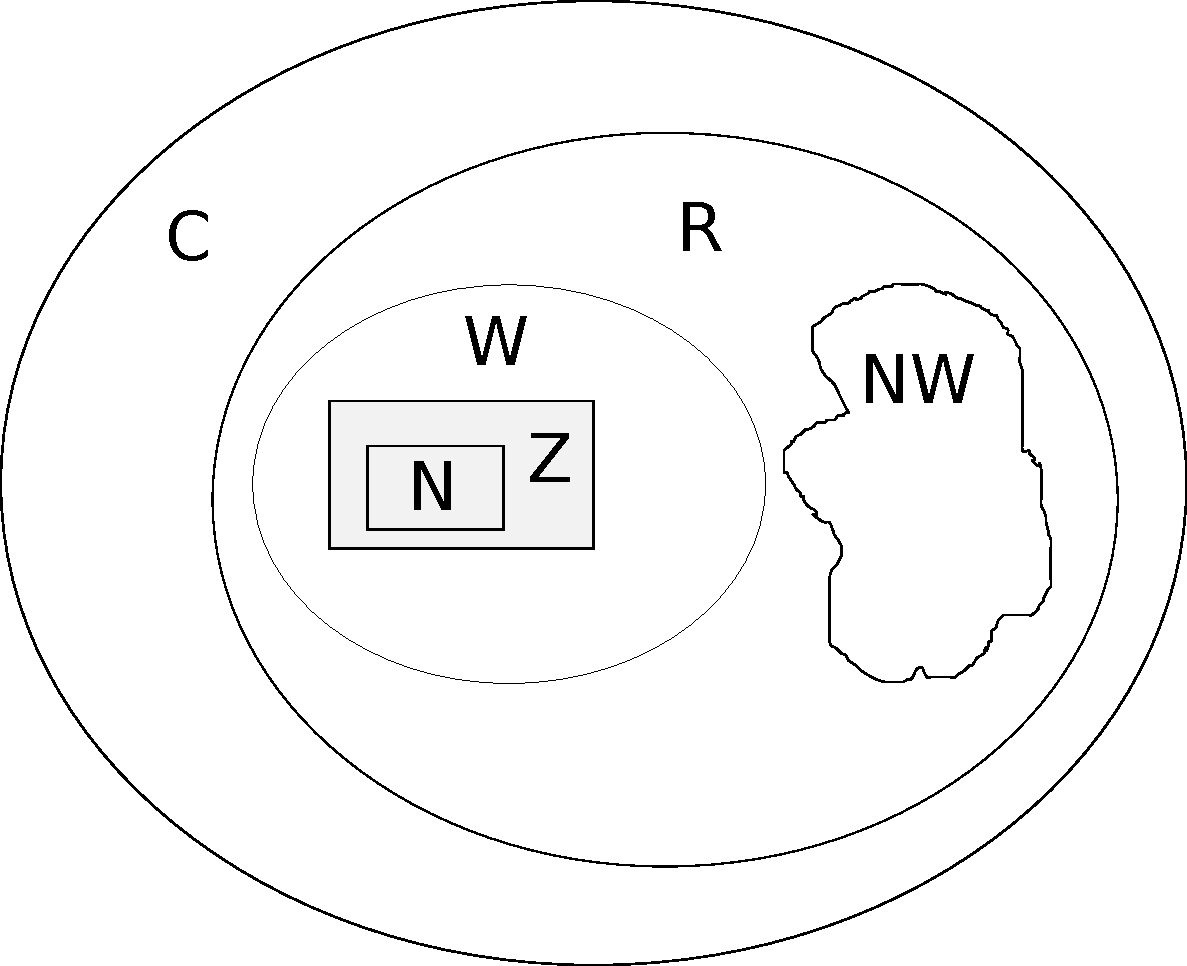
\includegraphics[width=0.70\textwidth]{drawing.pdf}
	\caption{Liczby zespolone}
	\label{fig:rozm}
\end{figure}

\section{Postać algebraiczna (kanoniczna)}
Każdą liczbę zespoloną z można zapisać w postaci $$z=a+bi$$, gdzie a i b są pewnymi liczbami rzeczywistymi oraz i jest tzw. jednostką urojoną, tj. i jest jednym z dwóch elementów zbioru liczb zespolonych, spełniającym warunek $i^2=-1$ (drugim elementem jest -i). Spotyka się czasami zapis $i=\sqrt{-1}$, który nie jest formalnie poprawny ze względu na fakt, że również $(-i)^2=-1$, jest on jednak uznawany za pewien skrót myślowy i powszechnie akceptowany.

Postać $z=a+bi$ nazywana jest postacią algebraiczną (albo kanoniczną) liczby zespolonej z.

Dla liczby $z=a+bi$ definiuje się jej
\begin{itemize}
\item część rzeczywistą (łac. pars realis) jako re $z = a$ (inne oznaczenia: $\Re z, Re, z$),
\item część urojoną (łac. pars imaginaria) jako im $z = b$ (inne oznaczenia: $\Im z, Im, z$).
\end{itemize}
Przykładowo liczba $\textbf{7 - 5i}$ jest liczbą zespoloną, której część rzeczywista wynosi 7, a część urojona -5. Liczby rzeczywiste są utożsamiane z liczbami zespolonymi o części urojonej równej 0.

Liczby postaci $z = 0 + bi$ nazywa się liczbami urojonymi.
\subsection{Zapis alternatywny}
W zastosowaniach fizycznych, elektrycznych, elektrotechnicznych itp. zapis $z = a + bi$ może okazać się mylący z powodu wykorzystywania w tych dziedzinach litery \textrm{\Large{i}} do innych celów, np. chwilowego natężenia prądu elektrycznego. Dlatego też stosuje się zapis niepowodujący podobnych kłopotów, mianowicie $z = a + jb$, w którym to j oznacza jednostkę urojoną.
\subsection{Równość}
Dwie liczby zespolone\footnote{To jest druga stopka}
 są równe wtedy i tylko wtedy, gdy ich części rzeczywiste i urojone są sobie równe. Innymi słowy, liczby zespolone postaci a + bi oraz c + di są sobie równe wtedy i tylko wtedy, gdy a = c oraz b = d.

\newpage
\subsection{Działania}
Dodawanie, odejmowanie i mnożenie liczb zespolonych w postaci algebraicznej wykonuje się tak samo jak odpowiednie operacje na wyrażeniach algebraicznych\footnote{To jest trzecia stopka}
, przy czym $i^2 = -1$

$(a + bi) \pm (c + di) = (a \pm c) + (b \pm d)i$
\newline
$(a + bi)(c + di) = ac + (bc + ad)i + bdi^2 = (ac - bd) + (bc + ad)i$
Aby podzielić przez siebie dwie liczby zespolone, wystarczy pomnożyć dzielną i dzielnik przez liczbę sprzężoną do dzielnika (analogicznie do usuwania niewymierności z mianownika w wyrażeniach algebraicznych):

$\frac{a + bi}{c + di} = \frac{(a + bi)(c - di)}{(c + di)(c - di)} = \frac{(ac + bd) + (bc - ad)i}{c^2 + d^2}$
\section{Przejście odwrotne}
$|z| = \sqrt{a^2 + b^2}$
\newline
$\gamma=$
$\begin{cases}
	arctg \frac{b}{a}, &\text{dla } a > 0\\
	arctg \frac{b}{a} + \pi, &\text{dla } a < 0 \text{ oraz } b \geq 0\\
	arctg \frac{b}{a} - \pi, &\text{dla } a < 0 \text{ oraz } b < 0\\
	+\frac{\pi}{2}, &\text{dla } a = 0 \text{ oraz } b > 0\\
	-\frac{\pi}{2}, &\text{dla } a = 0 \text{ oraz } b < 0\\
	niezdefiniowane, &\text{dla } a = 0 \text{ oraz } b = 0
\end{cases}$
\newpage
\section{tabele}
\begin{table}[htbp]
	\centering
		\begin{tabular}{|c|c|c|c|c|c|}
			\hline
			& 0 & $\frac{\pi}{6}$ & $\frac{\pi}{4}$ & $\frac{\pi}{3}$ & $\frac{\pi}{2}$ \\
			\hline
			& $0^\circ$ & $30^\circ$ & $45^\circ$ & $60^\circ$ & $90^\circ$ \\
			\hline
			$sin x$ & 0 & $\frac{1}{2}$ & $\frac{\sqrt{2}}{2}$ & $\frac{\sqrt{3}}{2}$ & 1 \\
			\hline
			$cos x$ & 1 & $\frac{\sqrt{3}}{2}$ & $\frac{\sqrt{2}}{2}$ & $\frac{1}{2}$ & 0 \\
			\hline
		\end{tabular}
	\caption{Macierz}
	\label{tab:Macierz}
\end{table}
\begin{figure}[htbp]
	\centering
		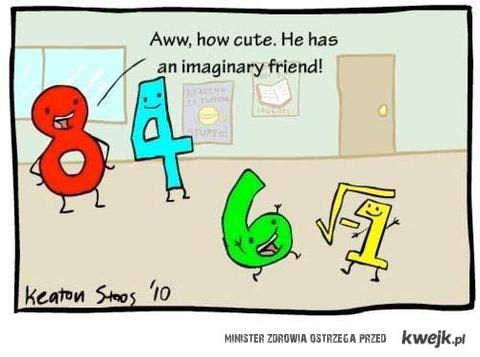
\includegraphics[width=0.70\textwidth]{licz.jpeg}
	\caption{Heheszki}
	\label{fig:licz}
\end{figure}

\begin{thebibliography}{99}
\item \url{http://www.matematyka.pl/latex.htm/}
\item \url{http://pl.wikipedia.org/wiki/Liczby_zespolone/}
\item \url{http://pl.wikibooks.org/wiki/LaTeX/Zarządzanie_bibliografią/}
\item \url{http://pl.wikibooks.org/wiki/LaTeX/Tabele/}
\item \url{http://pl.wikibooks.org/wiki/LaTeX/Zaczynamy/}
\end{thebibliography}
\end{document}